\documentclass[aspectratio=169]{beamer}
\usetheme{Madrid}
\usecolortheme{seahorse}
\usepackage{hyperref}
\usepackage{amsmath,amssymb}
\usepackage{tikz}
\usetikzlibrary{arrows.meta,positioning,shapes.geometric}
\usepackage{xcolor}

\title{From Chaos to Certificates}
\subtitle{How random AI dots became a barrier-synthesis verification system}
\author{Halley Young}
\date{March 2026}

\setbeamertemplate{navigation symbols}{}
\setbeamertemplate{footline}[frame number]

\newcommand{\bendtag}[1]{\textcolor{blue!70!black}{\textbf{How we bent it:} #1}}
\newcommand{\slottag}[1]{\textcolor{teal!70!black}{\textbf{Barrier slot:} #1}}

\begin{document}

\begin{frame}
\titlepage
\end{frame}

\begin{frame}{1. The crazy path (honest version)}
\begin{itemize}
  \item We did \textbf{not} start with a clean theorem-first architecture
  \item We started with many AI-generated, half-useful ideas (``dots'')
  \item Most dots were wrong, overfit, or non-executable
  \item The winning move: force every dot through executable semantics + regression pressure
  \item Surviving dots connected into one interface: \textbf{barrier obligations}
\end{itemize}
\end{frame}

\begin{frame}{2. Dot cloud \(\rightarrow\) connected system}
\begin{center}
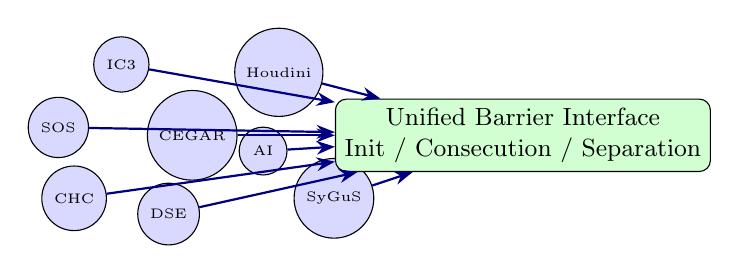
\begin{tikzpicture}[node distance=0.9cm,
  dot/.style={circle,draw,fill=blue!15,minimum size=0.42cm,font=\tiny},
  core/.style={rounded corners,draw,fill=green!18,minimum width=2.8cm,minimum height=0.8cm,font=\small,align=center}]

\node[dot] (d1) at (0,1.2) {SOS};
\node[dot] (d2) at (0.8,2.0) {IC3};
\node[dot] (d3) at (1.7,1.1) {CEGAR};
\node[dot] (d4) at (0.2,0.3) {CHC};
\node[dot] (d5) at (1.4,0.1) {DSE};
\node[dot] (d6) at (2.6,0.9) {AI};
\node[dot] (d7) at (2.8,1.9) {Houdini};
\node[dot] (d8) at (3.5,0.3) {SyGuS};

\node[core] (core) at (5.9,1.1) {Unified Barrier Interface\\Init / Consecution / Separation};

\foreach \x in {d1,d2,d3,d4,d5,d6,d7,d8}{\draw[-{Stealth},thick,blue!50!black] (\x) -- (core);}

\end{tikzpicture}
\end{center}
\begin{itemize}
  \item We kept ideas only if they discharged one barrier obligation or refined template search
\end{itemize}
\end{frame}

\begin{frame}{3. Why barrier synthesis was the right center of gravity}
\begin{itemize}
  \item It gives one testable contract across many methods:
  \[
  \forall s\in S_0: B(s)\ge\epsilon,\quad
  B(s)\ge0 \wedge T(s,s')\Rightarrow B(s')\ge0,\quad
  \forall s\in U: B(s)\le-\epsilon
  \]
  \item Every method can be judged by one question: which obligation does it help prove?
  \item Failure is informative: no silent drop, just reroute to the next method
  \item This turned ``paper zoo'' into a coherent portfolio
\end{itemize}
\end{frame}

\begin{frame}{4. Why useful vs existing approaches}
\begin{columns}
\begin{column}{0.48\textwidth}
\textbf{Existing (single-method):}
\begin{itemize}
  \item Pattern-only SAST: fast, noisy
  \item Pure symbolic only: path explosion
  \item Pure AI ranking: weak guarantees
  \item Single-solver FM: brittle on method mismatch
\end{itemize}
\end{column}
\begin{column}{0.48\textwidth}
\textbf{Barrier-centered portfolio:}
\begin{itemize}
  \item Shared proof interface
  \item Multiple orthogonal proof routes
  \item Explicit UNKNOWN policy
  \item Proof/witness artifacts in SARIF
\end{itemize}
\end{column}
\end{columns}
\vspace{0.3em}
\begin{block}{Operational value}
Lower false-positive load \emph{without} pretending every case is decidable.
\end{block}
\end{frame}

\begin{frame}{5. One bug-class as polynomial invariant}
\textbf{Bug class: DIV\_ZERO at a guarded site}
\begin{itemize}
  \item Program shape: \texttt{if den > 0: return num / den}
  \item Choose state variable: \(x = den\)
  \item Unsafe set: \(U(x) \equiv (x=0)\)
  \item Candidate barrier: \(B(x)=x-\tfrac{1}{2}\)
\end{itemize}
\begin{block}{Check obligations}
\begin{itemize}
  \item Init at division-reachable entry: \(x\ge1 \Rightarrow B(x)\ge\tfrac{1}{2}\)
  \item Consecution under guard-preserving transitions: \(x\ge1\Rightarrow x'\ge1\Rightarrow B(x')\ge\tfrac{1}{2}\)
  \item Separation: \(x=0\Rightarrow B(x)=-\tfrac{1}{2}<0\)
\end{itemize}
\end{block}
\end{frame}

\begin{frame}{6. How this maps to elimination}
\begin{itemize}
  \item Synthesis finds coefficients for \(B\)
  \item Solver validates all three obligations on encoded transition semantics
  \item If valid: candidate is provably unreachable (FP eliminated)
  \item If invalid/UNKNOWN: keep candidate, escalate portfolio
\end{itemize}
\begin{block}{Important}
Barrier synthesis is a \textbf{proof-producing filter}, not a magic one-shot classifier.
\end{block}
\end{frame}

\begin{frame}{6b. Contracts: why they matter in barrier theory}
\begin{itemize}
  \item Real Python verification includes unknown/external calls (e.g., \texttt{torch.*})
  \item Without contracts, call effects are too unconstrained \(\Rightarrow\) consecution collapses into UNKNOWN
  \item A contract gives a conservative callable summary:
  \[
  C_f: \text{Pre}(x)\Rightarrow \text{Post}(x,x')
  \]
  \item We inject \(C_f\) into transition relation as call-edge semantics
  \item Then barrier obligations are checked over \(T_{\text{prog}}\land C_f\), not over wishful behavior
\end{itemize}
\end{frame}

\begin{frame}{6c. PyTorch-style contract example}
\textbf{Example: \texttt{y = torch.clamp(x, min=0)}}
\begin{itemize}
  \item \textbf{Pre:} \(x\in\mathbb{R}^n\), finite tensor, known dtype family
  \item \textbf{Post:} \(\forall i,\ y_i\ge 0\) and \(y_i = \max(x_i,0)\)
  \item \textbf{Shape contract:} \(\text{shape}(y)=\text{shape}(x)\)
  \item \textbf{Effect contract:} no mutation of unrelated program state
\end{itemize}
\begin{block}{Barrier consequence}
If safety needs \(x_i\ge 0\) after this call, the contract makes that property solver-visible and usable in consecution.
\end{block}
\end{frame}

\begin{frame}{6d. Contracts inside obligations}
\begin{itemize}
  \item \textbf{Init with contracts:} include library preconditions in entry assumptions
  \item \textbf{Consecution with contracts:}
  \[
  B(s)\ge0\wedge T_{\text{prog}}(s,s')\wedge C_{\text{calls}}(s,s')\Rightarrow B(s')\ge0
  \]
  \item \textbf{Separation with contracts:} exclude unsafe states reachable only via contract-violating paths
  \item Contract quality controls precision:
  \begin{itemize}
    \item Too weak \(\Rightarrow\) more UNKNOWN/SAT survivors
    \item Unsound \(\Rightarrow\) invalid proof risk (forbidden)
    \item Conservative + checkable \(\Rightarrow\) safe elimination
  \end{itemize}
\end{itemize}
\end{frame}

\begin{frame}{7. 20 papers, one per slide: mapping rule}
\begin{itemize}
  \item For each paper we state:
  \begin{enumerate}
    \item Native contribution
    \item Exactly how we \textbf{bent} it into our barrier workflow
    \item Which barrier obligation/phase it serves
  \end{enumerate}
  \item ``Bent'' means adaptation from original domain assumptions to executable Python verification constraints
\end{itemize}
\end{frame}

\begin{frame}[t,shrink=8]{8. Paper 1/20 — Stengle 1974 (Positivstellensatz)}
\begin{itemize}
  \item \textbf{Native idea:} semialgebraic infeasibility has algebraic certificates
  \item \bendtag{Restrict to finite polynomial templates + Archimedean-style bounded domains from program guards}
  \item \slottag{Existence basis for separation certifiability}
\end{itemize}
\end{frame}

\begin{frame}[t,shrink=8]{9. Paper 2/20 — Parrilo 2000 (SOS programming)}
\begin{itemize}
  \item \textbf{Native idea:} positivity via SOS \(\Leftrightarrow\) SDP Gram matrix
  \item \bendtag{Use low-degree monomial bases derived from symbolic state projections instead of global algebraic variable sets}
  \item \slottag{Compute candidate \(B\) coefficients for init/sep constraints}
\end{itemize}
\end{frame}

\begin{frame}[t,shrink=8]{10. Paper 3/20 — Lasserre 2001 (moment hierarchy)}
\begin{itemize}
  \item \textbf{Native idea:} degree hierarchy converges to global polynomial optimum
  \item \bendtag{Turn hierarchy into budgeted escalation ladder: degree-2 \(\rightarrow\) degree-4 only when lower tier fails}
  \item \slottag{Controlled refinement when simple certificates fail}
\end{itemize}
\end{frame}

\begin{frame}[t,shrink=8]{11. Paper 4/20 — Prajna \& Jadbabaie 2004}
\begin{itemize}
  \item \textbf{Native idea:} barrier certificate obligations for dynamical safety
  \item \bendtag{Replace continuous dynamics state with bytecode transition-system state tuple \((pc,\rho,h,\tau,\kappa,e,\Phi)\)}
  \item \slottag{Canonical init/consecution/separation interface}
\end{itemize}
\end{frame}

\begin{frame}[t,shrink=8]{12. Paper 5/20 — Prajna et al. 2007 (stochastic barriers)}
\begin{itemize}
  \item \textbf{Native idea:} expectation-based barrier conditions under probabilistic dynamics
  \item \bendtag{Use expectation-style reasoning for uncertainty scoring paths, while keeping deterministic proof gate for elimination}
  \item \slottag{Risk-aware extension around consecution}
\end{itemize}
\end{frame}

\begin{frame}[t,shrink=8]{13. Paper 6/20 — Ahmadi \& Majumdar 2019 (DSOS/SDSOS)}
\begin{itemize}
  \item \textbf{Native idea:} LP/SOCP relaxations of SOS cone for speed
  \item \bendtag{Front-load DSOS tier in CI for throughput; escalate to full SDP only on failure}
  \item \slottag{Fast separation/invariant candidate screening}
\end{itemize}
\end{frame}

\begin{frame}[t,shrink=8]{14. Paper 7/20 — Waki et al. 2006 (correlative sparsity)}
\begin{itemize}
  \item \textbf{Native idea:} exploit sparse variable correlation in polynomial optimization
  \item \bendtag{Build certificate subproblems on localized variable clusters from dataflow slices}
  \item \slottag{Scalable separation checks for larger functions}
\end{itemize}
\end{frame}

\begin{frame}[t,shrink=8]{15. Paper 8/20 — Ames et al. 2019 (CBF survey)}
\begin{itemize}
  \item \textbf{Native idea:} control barrier function condition \(\dot{B}\ge-\alpha(B)\)
  \item \bendtag{Translate slope condition intuition into discrete successor condition \(B(s')\ge0\) contracts for unknown calls}
  \item \slottag{Consecution intuition + contract over-approximation}
\end{itemize}
\end{frame}

\begin{frame}[t,shrink=8]{16. Paper 9/20 — Sheeran et al. 2000 (k-induction)}
\begin{itemize}
  \item \textbf{Native idea:} SAT-based base+step proof up to depth \(k\)
  \item \bendtag{Use as fallback consecution checker when polynomial template quality is low}
  \item \slottag{Bounded-to-inductive consecution discharge}
\end{itemize}
\end{frame}

\begin{frame}[t,shrink=8]{17. Paper 10/20 — Bradley 2011 (IC3)}
\begin{itemize}
  \item \textbf{Native idea:} frame-based inductive clause strengthening
  \item \bendtag{Interpret learned frame conjunction as implicit non-polynomial barrier surface}
  \item \slottag{Consecution via clause barrier (implicit \(B\))}
\end{itemize}
\end{frame}

\begin{frame}[t,shrink=8]{18. Paper 11/20 — Een et al. 2011 (PDR)}
\begin{itemize}
  \item \textbf{Native idea:} industrial-strength IC3 with generalized blocking
  \item \bendtag{Serialize blocking clause progression as auditable proof artifact for SARIF evidence}
  \item \slottag{Operational consecution proof path}
\end{itemize}
\end{frame}

\begin{frame}[t,shrink=8]{19. Paper 12/20 — Gurfinkel et al. 2015 (SeaHorn/CHC)}
\begin{itemize}
  \item \textbf{Native idea:} software safety as constrained Horn clauses
  \item \bendtag{Encode interprocedural summaries as CHC predicates tied to barrier obligations at call boundaries}
  \item \slottag{Consecution across function boundaries}
\end{itemize}
\end{frame}

\begin{frame}[t,shrink=8]{20. Paper 13/20 — Clarke et al. 2000 (CEGAR)}
\begin{itemize}
  \item \textbf{Native idea:} refine abstraction using spurious counterexamples
  \item \bendtag{Treat failed barrier obligations as template counterexamples; add monomials/constraints only where failure occurred}
  \item \slottag{Template refinement loop}
\end{itemize}
\end{frame}

\begin{frame}[t,shrink=8]{21. Paper 14/20 — Ball et al. 2001 (SLAM)}
\begin{itemize}
  \item \textbf{Native idea:} predicate abstraction + CEGAR at industrial scale
  \item \bendtag{Mine predicates from symbolic path guards to seed barrier template terms}
  \item \slottag{Predicate source for refinement candidates}
\end{itemize}
\end{frame}

\begin{frame}[t,shrink=8]{22. Paper 15/20 — McMillan 2003 (Interpolants)}
\begin{itemize}
  \item \textbf{Native idea:} extract intermediate predicates from UNSAT proofs
  \item \bendtag{Convert interpolants into additional inequality features for next barrier synthesis round}
  \item \slottag{Counterexample-to-template repair}
\end{itemize}
\end{frame}

\begin{frame}[t,shrink=8]{23. Paper 16/20 — Henzinger et al. 2004 (Lazy abstraction)}
\begin{itemize}
  \item \textbf{Native idea:} refine only explored abstract regions
  \item \bendtag{Refine barrier template only for failing candidate/path cluster, not globally}
  \item \slottag{Localized synthesis cost control}
\end{itemize}
\end{frame}

\begin{frame}[t,shrink=8]{24. Paper 17/20 — Flanagan \& Leino 2001 (Houdini)}
\begin{itemize}
  \item \textbf{Native idea:} maximal inductive subset of candidate invariants
  \item \bendtag{Generate broad candidate coefficient/inequality family, prune with obligation counterexamples}
  \item \slottag{Invariant candidate curation before expensive solves}
\end{itemize}
\end{frame}

\begin{frame}[t,shrink=8]{25. Paper 18/20 — Garg et al. 2014 (ICE learning)}
\begin{itemize}
  \item \textbf{Native idea:} learn invariants from positive/negative/implication examples
  \item \bendtag{Use obligation-failure states as implication examples to learn better barrier feature combinations}
  \item \slottag{Data-driven invariant synthesis support}
\end{itemize}
\end{frame}

\begin{frame}[t,shrink=8]{26. Paper 19/20 — Alur et al. 2013 (SyGuS)}
\begin{itemize}
  \item \textbf{Native idea:} syntax-guided program/expression synthesis
  \item \bendtag{Constrain barrier template grammar (allowed monomials/predicates) for controllable search spaces}
  \item \slottag{Grammar-bounded certificate synthesis}
\end{itemize}
\end{frame}

\begin{frame}[t,shrink=8]{27. Paper 20/20 — Godefroid et al. 2005 (DART/concolic)}
\begin{itemize}
  \item \textbf{Native idea:} dynamic symbolic execution for concrete witness generation
  \item \bendtag{Use concolic as post-proof cross-check: confirm SAT survivors and reject spurious models from coarse abstractions}
  \item \slottag{Witness grounding after barrier/SMT uncertainty}
\end{itemize}
\end{frame}

\begin{frame}{28. What this gives us in practice}
\begin{itemize}
  \item One unifying certificate contract across 20 heterogeneous methods
  \item Better FP collapse than pattern-only or single-method pipelines
  \item Structured UNKNOWN handling instead of silent optimism
  \item Explainable outputs: each decision maps to obligation evidence
\end{itemize}
\end{frame}

\begin{frame}{29. Final notes for the audience}
\begin{itemize}
  \item The novelty is not ``invented one new theorem''
  \item The novelty is \textbf{integration discipline}: force random ideas into one falsifiable interface
  \item Barrier synthesis is useful because it converts method diversity into coherent proof plumbing
  \item AI helped generate dots; engineering connected the right dots
\end{itemize}
\end{frame}

\begin{frame}{30. Close}
\begin{center}
\Large
From slop to structure:\\
\vspace{0.3em}
\textbf{Init. Consecution. Separation.}\\
\vspace{0.6em}
\normalsize
Everything else is routing.
\end{center}
\end{frame}

\end{document}
